\documentclass[12pt]{article}
 
\usepackage[margin=1in]{geometry} 
\usepackage{amsmath,amsthm,amssymb}
\usepackage{graphicx}
\usepackage{tikz}
\usetikzlibrary{calc,patterns,angles,quotes}
 
\newcommand{\N}{\mathbb{N}}
\newcommand{\Z}{\mathbb{Z}}
\newcommand{\R}{\mathbb{R}}
\newcommand{\C}{\mathbb{C}}

\usepackage{mathtools}
\DeclarePairedDelimiter\ceil{\lceil}{\rceil}
\DeclarePairedDelimiter\floor{\left\lfloor}{\right\rfloor}
 
\usepackage{amsthm}
\newtheorem{proposition}{Proposition}
 
\begin{document}
 
% --------------------------------------------------------------
%                         Start here
% --------------------------------------------------------------
 
\title{Solutions to Exercise Sheet 1}
\author{Leif Van Holland \\ \\
\textsc{Discrete and Computational Geometry}}

\maketitle

\section*{Exercise 1}
\begin{proposition}[upper bound]
Let $\Gamma$ be the set of non-intersecting polygonal chains $C$ in the plane where the geometric dilation $\delta(C)>1$. Let $n$ be the number of vertices of $C$ and $P(C)$ be the number of pairs $p,q\in C$, where the geometric dilation of $C$ is attained an $p$ is a vertex of $C$. Then
\[P(C)\in O(n^2) \text{ if } C\in\Gamma.\]
\end{proposition}
\begin{proof}
From Lemma 2 we know, that for every pair $p,q\in C$ where $C$ attains maximum dilation, at least one of the points has to be a vertex of $C$. W.l.o.g., let $p$ be a vertex of $C$. Using the method described in the lecture, we can determine the maximum dilation of $C$ for every vertex-edge-pair $p,e$ by parameterizing $e$ as points $q(t)\in e, t\in I$ with $|I|=|e|$. This yields the following equation
\[\delta(p,q(t)) = \frac{t+|C_p^q|}{r(t)},\qquad r(t) := \sqrt{t^2-2\cos\beta|pq|t+|pq|^2} \]
and its derivative with respect to t
\begin{align}\delta'(p,q(t)) = \frac{r(t)-\frac{1}{2r(t)}(2t-2\cos\beta|pq|)(t+|C_p^q|)}{r(t)^2}.
\label{deltaderiv}
\end{align}
Roots of \eqref{deltaderiv} provide points $q(t)$ that maximize the dilation of $C$. We can see with
\begin{align*}
    0 = \delta'(p,q(t))
    \iff 0 = t^2 - 2 \cos\beta |pq|t+|pq|^2-\frac{1}{2}(2t-2\cos\beta|pq|)(t+|C_p^q|), 
\end{align*}
that \eqref{deltaderiv} has at most two roots $t_1, t_2$. Therefore, every of the $n\cdot(n-1)$ vertex-edge-pairs contributes at most two pairs $(p,q(t_1))$ and $(p,q(t_2))$, where maximum dilation of $C$ is attained. In other words
\[
P(C) < 2\cdot n(n-1) \in O(n^2)
\]
\end{proof}

\begin{proposition}[lower bound] Let $C\in\Gamma$. Then the following statement holds
\[P(C) \in \Omega(n^2).\]
\end{proposition}
\begin{proof}
We prove this by giving a construction scheme for a chain $C=(p_1, ..., p_n), n\geq2$. In the following $p\perp q$ denotes that $p$ is perpendicular to $q$.
\begin{itemize}
    \item For $i=1$, choose any $p_1\in\R^2$.
    \item For $i=2$, choose any $p_2\in\R^2$ with $|C_1^2| = 1$.
    \item For $i=3$, choose $p_3\in\R^2$ so that $C_1^2 \perp C_2^3$ and $|C_2^3| = 1$
    \item For $i>3$, choose $p_i\in\R^2$ so that $C_{i-2}^{i-1} \perp C_{i-1}^i, |p_{i-2}p_i| = |p_{i-3}p_{i-1}|$ and $|C_{i-1}^i| = 1$.
\end{itemize}
Following this scheme, $C$ might looks as follows:

\begin{figure}[h]
\centering
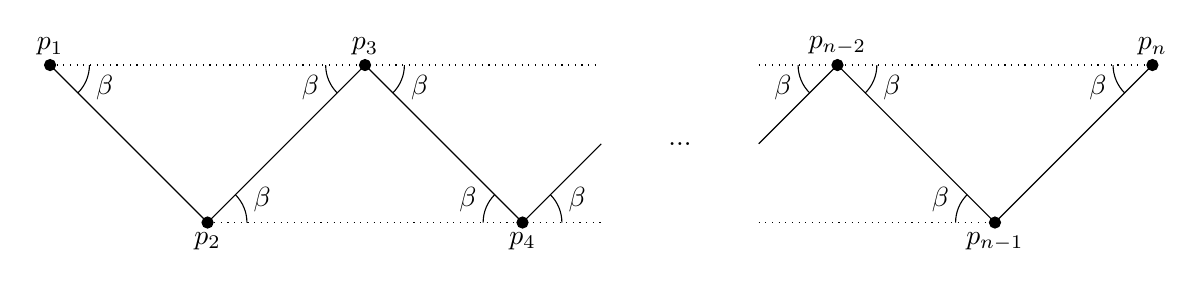
\begin{tikzpicture}

\coordinate (p1) at (0,0);
\coordinate (p2) at (2,-2);
\coordinate (p3) at (4,0);
\coordinate (p4) at (6,-2);
\coordinate (p4a) at (7,-1);
\coordinate (pn2a) at (9,-1);
\coordinate (pn2) at (10,0);
\coordinate (pn1) at (12,-2);
\coordinate (pn) at (14,0);

\draw (p1) -- (p2) -- (p3) -- (p4) -- (p4a);

\filldraw[black] (p1) circle (2pt) node[anchor=south] {$p_1$};
\pic [draw, -, "$\beta$", angle eccentricity=1.5] {angle = p2--p1--p3};

\filldraw[black] (p2) circle (2pt) node[anchor=north] {$p_2$};
\pic [draw, -, "$\beta$", angle eccentricity=1.5] {angle = p4--p2--p3};

\filldraw[black] (p3) circle (2pt) node[anchor=south] {$p_3$};
\pic [draw, -, "$\beta$", angle eccentricity=1.5] {angle = p4--p3--pn2};
\pic [draw, -, "$\beta$", angle eccentricity=1.5] {angle = p1--p3--p2};

\filldraw[black] (p4) circle (2pt) node[anchor=north] {$p_4$};
\pic [draw, -, "$\beta$", angle eccentricity=1.5] {angle = p3--p4--p2};
\pic [draw, -, "$\beta$", angle eccentricity=1.5] {angle = pn1--p4--p4a};

\node at (8,-1) {...};
\draw (pn2a) -- (pn2) -- (pn1) -- (pn);

\filldraw[black] (pn2) circle (2pt) node[anchor=south] {$p_{n-2}$};
\pic [draw, -, "$\beta$", angle eccentricity=1.5] {angle = p3--pn2--pn2a};
\pic [draw, -, "$\beta$", angle eccentricity=1.5] {angle = pn1--pn2--pn};

\filldraw[black] (pn1) circle (2pt) node[anchor=north] {$p_{n-1}$};
\pic [draw, -, "$\beta$", angle eccentricity=1.5] {angle = pn2--pn1--p4};

\filldraw[black] (pn) circle (2pt) node[anchor=south] {$p_n$};
\pic [draw, -, "$\beta$", angle eccentricity=1.5] {angle = pn2--pn--pn1};

\draw[dotted] (p1) -- (7,0);
\draw[dotted] (9,0) -- (pn);
\draw[dotted] (p2) -- (7,-2);
\draw[dotted] (9,-2) -- (pn1);
\end{tikzpicture}
\end{figure}

Observe that this construction causes all vertices with odd indices lie on a line segment $l_{odd}$ and all vertices with even indices lie on another line $l_{even}$. From Lemma 1 we know that
\begin{align}
    p,q\in C \text{ attain a locally maximal dilation } \iff \cos \beta = \frac{-|pq|}{|C_p^q|}
\end{align}
where $\beta$ is the angle enclosed by the edge $e\in C$ with $p\in e$ that is on the path to $q$ and the line segment $pq$. W.l.o.g. we will only consider vertices with an odd index for now (the construction is completely analogous for even indices). All these vertices lie on the line segment $l_{odd}$. Let $p_i, p_j$ be two of these vertices and w.l.o.g $i<j$. Let $\beta$ be the angle defined like above.

From the construction scheme we can derive that
\begin{itemize}
    \item[(i)] $|p_i p_{i+1}| = |p_{i+1}p_{i+2}| = 1$,
    \item[(ii)] $p_i p_{i+1}, p_{i+2}$ form a triangle $T$ where $p_i p_{i+1} \perp p_{i+1}p_{i+2}$, $p_i p_{i+2}$ is the hypotenuse of $T$ and $p_i p_{i+2} \subset l_{odd}$ and $|p_i p_{i+2}| = \sqrt{2}$ and
    \item[(iii)] $\beta \overset{\text{(ii)}}{=} \frac{\pi}{4}$.
    \item[(iv)] $|p_i p_j| = \sqrt{2}\cdot\left(\frac{j-i}{2}\right)$ and $|C_{p_i}^{p_j}| = j-i$
\end{itemize}
From these observations we can conclude, that
\[\frac{-|p_i p_j|}{|C_{p_i}^{p_j}|}\overset{\text{(iv)}}{=}\frac{-\sqrt{2}\cdot\frac{1}{2}(j-i)}{(j-i)} = -\frac{1}{\sqrt{2}} = \cos\frac{\pi}{4} \overset{\text{(iii)}}{=} \cos{\beta}.  \]
From (2) we now know, that the dilation is locally maximal and this result was obtained regardless of the choice of $i$ and $j$. Therefore we get
\[ \delta(p_i,p_j) = \delta(C) = \sqrt{2}\]This means that for every vertex $p\in C$, we find $(\floor{\frac{n}{2}}-1)$ other vertices $p_j$ with $\delta(C) = \delta(p_i,p_j) = \sqrt{2}$. All in all, this amounts to
\[ P(C) = n\cdot\left(\floor{\frac{n}{2}}-1\right) \in \Omega(n^2) \]
\end{proof}

\begin{proposition}
If $C\not\in\Gamma$ is an arbitrary non-intersecting polygonal chain, then $P(C) = \infty$.
\end{proposition}
\begin{proof} 
By definition, $C\not\in\Gamma$ implies that $\delta(C)\leq 1$. Because for all $p,q\in C$, $|C_p^q| \geq |pq|$ always holds, we can conclude that
\[\delta(C)=\max_{\substack{p,q\in C\\p\neq q}} \frac{|C_p^q|}{|pq|}=1\]
and more specifically
\[\forall p,q\in C, p\neq q: \delta_C(p,q) = \delta(C) = 1.\]
There is an infinite amount of choices for $p$ and $q$, therefore \[P(C) = \infty.\]
\end{proof}
 
% --------------------------------------------------------------
%     You don't have to mess with anything below this line.
% --------------------------------------------------------------
 
\end{document}